%%%%%%%%%%%%%%%%%%%%%%%%%%%%%%%%%%%%%%%%%%%%%%%%%%%%%%%%%%%%%%%%%%%%%%%%%%%%%%%%
%%%%%%%%%%%%%%%%%%%%%%%%%%%%%%%%%%%%%%%%%%%%%%%%%%%%%%%%%%%%%%%%%%%%%%%%%%%%%%%%
%%                                                                            %%
%% thesistemplate.tex version 3.20 (2018/08/31)                               %%
%% The LaTeX template file to be used with the aaltothesis.sty (version 3.20) %%
%% style file.                                                                %%
%% This package requires pdfx.sty v. 1.5.84 (2017/05/18) or newer.            %%
%%                                                                            %%
%% This is licensed under the terms of the MIT license below.                 %%
%%                                                                            %%
%% Written by Luis R.J. Costa.                                                %%
%% Currently developed at the Learning Services of Aalto University School of %%
%% Electrical Engineering by Luis R.J. Costa since May 2017.                  %%
%%                                                                            %%
%% Copyright 2017-2018, by Luis R.J. Costa, luis.costa@aalto.fi,              %%
%% Copyright 2017-2018 Swedish translations in aaltothesis.cls by Elisabeth   %%
%% Nyberg, elisabeth.nyberg@aalto.fi and Henrik Wallén,                       %%
%% henrik.wallen@aalto.fi.                                                    %%
%% Copyright 2017-2018 Finnish documentation in the template opinnatepohja.tex%%
%% by Perttu Puska, perttu.puska@aalto.fi, and Luis R.J. Costa.               %%
%% Copyright 2018 English template thesistemplate.tex by Luis R.J. Costa.     %%
%% Copyright 2018 Swedish template kandidatarbetsbotten.tex by Henrik Wallen. %%
%%                                                                            %%
%% Permission is hereby granted, free of charge, to any person obtaining a    %%
%% copy of this software and associated documentation files (the "Software"), %%
%% to deal in the Software without restriction, including without limitation  %%
%% the rights to use, copy, modify, merge, publish, distribute, sublicense,   %%
%% and/or sell copies of the Software, and to permit persons to whom the      %%
%% Software is furnished to do so, subject to the following conditions:       %%
%% The above copyright notice and this permission notice shall be included in %%
%% all copies or substantial portions of the Software.                        %%
%% THE SOFTWARE IS PROVIDED "AS IS", WITHOUT WARRANTY OF ANY KIND, EXPRESS OR %%
%% IMPLIED, INCLUDING BUT NOT LIMITED TO THE WARRANTIES OF MERCHANTABILITY,   %%
%% FITNESS FOR A PARTICULAR PURPOSE AND NONINFRINGEMENT. IN NO EVENT SHALL    %%
%% THE AUTHORS OR COPYRIGHT HOLDERS BE LIABLE FOR ANY CLAIM, DAMAGES OR OTHER %%
%% LIABILITY, WHETHER IN AN ACTION OF CONTRACT, TORT OR OTHERWISE, ARISING    %%
%% FROM, OUT OF OR IN CONNECTION WITH THE SOFTWARE OR THE USE OR OTHER        %%
%% DEALINGS IN THE SOFTWARE.                                                  %%
%%                                                                            %%
%%                                                                            %%
%%%%%%%%%%%%%%%%%%%%%%%%%%%%%%%%%%%%%%%%%%%%%%%%%%%%%%%%%%%%%%%%%%%%%%%%%%%%%%%%
%%                                                                            %%
%%                                                                            %%
%% An example for writting your thesis using LaTeX                            %%
%% Original version and development work by Luis Costa, changes to the text   %% 
%% in the Finnish template by Perttu Puska.                                   %%
%% Support for Swedish added 15092014                                         %%
%% PDF/A-b support added on 15092017                                          %%
%% PDF/A-2 support added on 24042018                                          %%
%%                                                                            %%
%% This example consists of the files                                         %%
%%         thesistemplate.tex (version 3.20) (for text in English)            %%
%%         opinnaytepohja.tex (version 3.20) (for text in Finnish)            %%
%%         kandidatarbetsbotten.tex (version 1.00) (for text in Swedish)      %%
%%         aaltothesis.cls (versio 3.20)                                      %%
%%         kuva1.eps (graphics file)                                          %%
%%         kuva2.eps (graphics file)                                          %%
%%         kuva1.jpg (graphics file)                                          %%
%%         kuva2.jpg (graphics file)                                          %%
%%         kuva1.png (graphics file)                                          %%
%%         kuva2.png (graphics file)                                          %%
%%         kuva1.pdf (graphics file)                                          %%
%%         kuva2.pdf (graphics file)                                          %%
%%                                                                            %%
%%                                                                            %%
%% Typeset in Linux either with                                               %%
%% pdflatex: (recommended method)                                             %%
%%             $ pdflatex thesistemplate                                      %%
%%             $ pdflatex thesistemplate                                      %%
%%                                                                            %%
%%   The result is the file thesistemplate.pdf that is PDF/A compliant, if    %%
%%   you have chosen the proper \documenclass options (see comments below)    %%
%%   and your included graphics files have no problems.
%%                                                                            %%
%% Or                                                                         %%
%% latex: (this method is not recommended)                                    %%
%%             $ latex thesistemplate                                         %%
%%             $ latex thesistemplate                                         %%
%%                                                                            %%
%%   The result is the file thesistemplate.dvi, which is converted to ps      %%
%%   format as follows:                                                       %%
%%                                                                            %%
%%             $ dvips thesistemplate -o                                      %%
%%                                                                            %%
%%   and then to pdf as follows:                                              %%
%%                                                                            %%
%%             $ ps2pdf thesistemplate.ps                                     %%
%%                                                                            %%
%%   This pdf file is not PDF/A compliant. You must must make it so using,    %%
%%   e.g., Acrobat Pro or PDF-XChange.                                        %%
%%                                                                            %%
%%                                                                            %%
%% Explanatory comments in this example begin with the characters %%, and     %%
%% changes that the user can make with the character %                        %%
%%                                                                            %%
%%%%%%%%%%%%%%%%%%%%%%%%%%%%%%%%%%%%%%%%%%%%%%%%%%%%%%%%%%%%%%%%%%%%%%%%%%%%%%%%
%%%%%%%%%%%%%%%%%%%%%%%%%%%%%%%%%%%%%%%%%%%%%%%%%%%%%%%%%%%%%%%%%%%%%%%%%%%%%%%%
%%
%% WHAT is PDF/A
%%
%% PDF/A is the ISO-standardized version of the pdf. The standard's goal is to
%% ensure that he file is reproducable even after a long time. PDF/A differs
%% from pdf in that it allows only those pdf features that support long-term
%% archiving of a file. For example, PDF/A requires that all used fonts are
%% embedded in the file, whereas a normal pdf can contain only a link to the
%% fonts in the system of the reader of the file. PDF/A also requires, among
%% other things, data on colour definition and the encryption used.
%% Currently three PDF/A standards exist:
%% PDF/A-1: based on PDF 1.4, standard ISO19005-1, published in 2005.
%%          Includes all the requirements essential for long-term archiving.
%% PDF/A-2: based on PDF 1.7, standard ISO19005-2, published in 2011.
%%          In addition to the above, it supports embedding of OpenType fonts,
%%          transparency in the colour definition and digital signatures.
%% PDF/A-3: based on PDF 1.7, standard ISO19005-3, published in 2012.
%%          Differs from the above only in that it allows embedding of files in
%%          any format (e.g., xml, csv, cad, spreadsheet or wordprocessing
%%          formats) into the pdf file.
%% PDF/A-1 files are not necessarily PDF/A-2 -compatible and PDF/A-2 are not
%% necessarily PDF/A-1 -compatible.
%% All of the above PDF/A standards have two levels:
%% b: (basic) requires that the visual appearance of the document is reliably
%%    reproduceable.
%% a (accessible) in addition to the b-level requirements, specifies how
%%   accessible the pdf file is to assistive software, say, for the physically
%%   impaired.
%% For more details on PDF/A, see, e.g., https://en.wikipedia.org/wiki/PDF/A
%%
%%
%% WHICH PDF/A standard should my thesis conform to?
%%
%% Primarily to the PDF/A-1b standard. All the figures and graphs typically
%% use in thesis work do not require transparency features, a basic '2-D'
%% visualisation suffices. The font to be used are specified in this template
%% and they should not be changed. However, if you have figures where
%% transparency characteristics matter, use the PDF/A-2b standard. Do not use
%% the PDF/A-3b standard for your thesis.
%%
%%
%% WHAT graphics format can I use to produce my PDF/A compliant file?
%%
%% When using pdflatex to compile your work, use jpg, png or pdf files. You may
%% have PDF/A compliance problems with figures in pdf format. Do not use PDF/A
%% compliant graphics files.
%% If you decide to use latex to compile your work, the only acceptable file
%% format for your figure is eps. DO NOT use the ps format for your figures.

%% USE one of these:
%% * the first when using pdflatex, which directly typesets your document in the
%%   chosen pdf/a format and you want to publish your thesis online,

%% * the second when you want to print your thesis to bind it, or
%% * the third when producing a ps file and a pdf/a from it.
%%
\documentclass[english, 12pt, a4paper, sci, utf8, a-1b, online]{aaltothesis}
%\documentclass[english, 12pt, a4paper, elec, utf8, a-1b]{aaltothesis}
%\documentclass[english, 12pt, a4paper, elec, dvips, online]{aaltothesis}

%% Use the following options in the \documentclass macro above:
%% your school: arts, biz, chem, elec, eng, sci
%% the character encoding scheme used by your editor: utf8, latin1
%% thesis language: english, finnish, swedish
%% make an archiveable PDF/A-1b or PDF/A-2b compliant file: a-1b, a-2b
%%                    (with pdflatex, a normal pdf containing metadata is
%%                     produced without the a-*b option)
%% typeset in symmetric layout and blue hypertext for online publication: online
%%            (no option is the default, resulting in a wide margin on the
%%             binding side of the page and black hypertext)
%% two-sided printing: twoside (default is one-sided printing)
%%

%% Use one of these if you write in Finnish (see the Finnish template
%% opinnaytepohja.tex)
%\documentclass[finnish, 12pt, a4paper, elec, utf8, a-1b, online]{aaltothesis}
%\documentclass[finnish, 12pt, a4paper, elec, utf8, a-1b]{aaltothesis}
%\documentclass[finnish, 12pt, a4paper, elec, dvips, online]{aaltothesis}

\usepackage{graphicx}
\usepackage{tabularx}
\usepackage{natbib}
\usepackage{float}

%% Math fonts, symbols, and formatting; these are usually needed
\usepackage{amsfonts,amssymb,amsbsy,amsmath}

%% Change the school field to specify your school if the automatically set name
%% is wrong
% \university{aalto-yliopisto}
% \school{Sähkötekniikan korkeakoulu}

%% Edit to conform to your degree programme
%%
\degreeprogram{Computer, Communication and Information Sciences}
%%

%% Your major
%%
\major{Software and Service Engineering}
%%

%% Major subject code
%%
\code{SCI3043}
%%
 
%% Choose one of the three below
%%
%\univdegree{BSc}
\univdegree{MSc}
%\univdegree{Lic}
%%

%% Your name (self explanatory...)
%%
\thesisauthor{Anders Nylund}
%%

%% Your thesis title comes here and possibly again together with the Finnish or
%% Swedish abstract. Do not hyphenate the title, and avoid writing too long a
%% title. Should LaTeX typeset a long title unsatisfactorily, you mght have to
%% force a linebreak using the \\ control characters.
%% In this case...
%% Remember, the title should not be hyphenated!
%% A possible "and" in the title should not be the last word in the line, it
%% begins the next line.
%% Specify the title again without the linebreak characters in the optional
%% argument in box brackets. This is done because the title is part of the 
%% metadata in the pdf/a file, and the metadata cannot contain linebreaks.
%%
\thesistitle{Developer Experience}
%\thesistitle[Title of the thesis]{Title of\\ the thesis}
%%

%%
\place{Espoo}
%%

%% The date for the bachelor's thesis is the day it is presented
%%
\date{TBA}
%%

%% Thesis supervisor
%% Note the "\" character in the title after the period and before the space
%% and the following character string.
%% This is because the period is not the end of a sentence after which a
%% slightly longer space follows, but what is desired is a regular interword
%% space.
%%
\supervisor{Prof.\ Pirjo Professor}
%%

%% Advisor(s)---two at the most---of the thesis. Check with your supervisor how
%% many official advisors you can have.
%%
\advisor{Dr Alan Advisor}
%\advisor{MSc Sarah Scientist}
%%

%% Aaltologo: syntax:
%% \uselogo{aaltoRed|aaltoBlue|aaltoYellow|aaltoGray|aaltoGrayScale}{?|!|''}
%% The logo language is set to be the same as the thesis language.
%%
\uselogo{aaltoRed}{''}
%%

%% The English abstract:
%% All the details (name, title, etc.) on the abstract page appear as specified
%% above.
%% Thesis keywords:
%% Note! The keywords are separated using the \spc macro
%%
\keywords{Developer Experience\spc Software Projects}
%%

%% The abstract text. This text is included in the metadata of the pdf file as well
%% as the abstract page.
%%

\newcommand{\englishabstract}{The abstract in english}
\newcommand{\swedishabstract}{Sammandrag på svenska}

\thesisabstract{
  \englishabstract
}

%% Copyright text. Copyright of a work is with the creator/author of the work
%% regardless of whether the copyright mark is explicitly in the work or not.
%% You may, if you wish, publish your work under a Creative Commons license (see
%% creaticecommons.org), in which case the license text must be visible in the
%% work. Write here the copyright text you want. It is written into the metadata
%% of the pdf file as well.
%% Syntax:
%% \copyrigthtext{metadata text}{text visible on the page}
%% 
%% In the macro below, the text written in the metadata must have a \noexpand
%% macro before the \copyright special character, and macros (\copyright and
%% \year here) must be separated by the \ character (space chacter) from the
%% text that follows. The macros in the argument of the \copyrighttext macro
%% automatically insert the year and the author's name. (Note! \ThesisAuthor is
%% an internal macro of the aaltothesis.cls class file).
%% Of course, the same text could have simply been written as
%% \copyrighttext{Copyright \noexpand\copyright\ 2018 Eddie Engineer}
%% {Copyright \copyright{} 2018 Eddie Engineer}
%%
\copyrighttext{Copyright \noexpand\copyright\ \number\year\ \ThesisAuthor}
{Copyright \copyright{} \number\year{} \ThesisAuthor}

%% You can prevent LaTeX from writing into the xmpdata file (it contains all the 
%% metadata to be written into the pdf file) by setting the writexmpdata switch
%% to 'false'. This allows you to write the metadata in the correct format
%% directly into the file thesistemplate.xmpdata.
%\setboolean{writexmpdatafile}{false}

%% All that is printed on paper starts here
%%
\begin{document}

%% Create the coverpage
%%
\makecoverpage

%% Typeset the copyright text.
%% If you wish, you may leave out the copyright text from the human-readable
%% page of the pdf file. This may seem like a attractive idea for the printed
%% document especially if "Copyright (c) yyyy Eddie Engineer" is the only text
%% on the page. However, the recommendation is to print this copyright text.
%%
\makecopyrightpage

%% Note that when writting your thesis in English, place the English abstract
%% first followed by the possible Finnish or Swedish abstract.

%% Abstract text
%% All the details (name, title, etc.) on the abstract page appear as specified
%% above.
%%
\begin{abstractpage}[english]
  \englishabstract
\end{abstractpage}

%% The text in the \thesisabstract macro is stored in the macro \abstractext, so
%% you can use the text metadata abstract directly as follows:
%%
%\begin{abstractpage}[english]
%	\abstracttext{}
%\end{abstractpage}

%% Force a new page so that the possible Finnish or Swedish abstract does not
%% begin on the same page
%%
% \newpage
% %%
% %% Abstract in Finnish.  Delete if you don't need it. 
% %%
% \thesistitle{Opinnäyteen otsikko}
% \supervisor{Prof.\ Pirjo Professori}
% \advisor{TkT Alan Advisor}
% \degreeprogram{Elektroniikka ja sähkötekniikka}
% %\department{Elektroniikan ja nanotekniikan laitos}
% \major{Sopiva pääaine}
% %% The keywords need not be separated by \spc now.
% \keywords{Vastus, resistanssi, lämpötila}
% %% Abstract text
% \begin{abstractpage}[finnish]
%   Tiivistelmässä on lyhyt selvitys
%   kirjoituksen tärkeimmästä sisällöstä: mitä ja miten on tutkittu,
%   sekä mitä tuloksia on saatu. 
% \end{abstractpage}

%% Force new page so that the Swedish abstract starts from a new page
\newpage

%% Swedish abstract. Delete it if you don't need it. 
%% 
\thesistitle{Developer Experience}
\supervisor{Prof.\ Pirjo Professori}
\advisor{TkD Alan Advisor} %
\degreeprogram{Computer, Communication and Information Sciences}
\department{Institutionen för radiovetenskap och -teknik}%
%% Abstract keywords
\keywords{Nyckelord på svenska, temperatur}
%% Abstract text
\begin{abstractpage}[swedish]
  \swedishabstract
\end{abstractpage}

%% Preface
%%
%% This section is optional. Remove it if you do not want a preface.
\mysection{Preface}
I want to thank Professor Pirjo Professori and my instructor Dr Alan Advisor for their good and poor guidance.

\vspace{5cm}
Otaniemi, Date to te announced

\vspace{5mm}
{\hfill Anders Nylund \hspace{1cm}}

%% Force a new page after the preface
%%
\newpage


%% Table of contents. 
%%
\thesistableofcontents

%% Symbols and abbreviations
\mysection{Thesis dictionary}

\begin{tabular}{ll}
  DX    & Developer Experience               \\
  UX    & User Experience                    \\
  IDE   & Integrated Development Environment \\
  IM    & Intrinsic Motivation               \\
  EM    & Extrinsic Motivation               \\
  HCI   & Human Computer Interaction         \\
  API   & Application Programming Interface  \\
  SLR   & Systematic Literature Review       \\
  MLR   & Multivocal Literature Review       \\
  GL    & Grey Literature                    \\
  SE    & Software Engineering               \\
  MSECO & Mobile Software Ecosystem          \\
\end{tabular}

%% \clearpage is similar to \newpage, but it also flushes the floats (figures
%% and tables).
%%
\cleardoublepage
\section{Introduction}

Software engineering and development is a complex practice that requires both technical and social skills. Compared to other engineering professions, software engineering is still in early stages. The best practices are still evolving, new ideas are coming and previous ideals are discarded.

Developing and creating software is a social activity that requires both technical and social skills from the developers. Deep technical skills and understanding is required to be able to implemented the required features. Software products are however used by people, and therefore it is a requirement to understand how social interactions work. Software is also most of the times

Software developers are in an interesting role where they are both creators and designers when they write the logic that makes up the product. Meantime they are also users of tools that they use to create the product. Developers using a software product that helps in their creative design work will create an user experience for them. Human Computer Interaction (HCI), a traditional field of research, studies the interface and interaction between computers and humans. User Experience (UX) is another field of research. UX includes the aspects of HCI, but on top of that includes also emotions and the user's perceptions of the product. UX can be seen as a more hedonic than a pragmatic approach of studying and understanding the usage of a software product.

In recent academic research and internet articles a concept called Developer Experience (DX) has gotten traction. DX is a term that explains how developers experience their development environments, both technically and socially. The same way as User Experience (UX) is considering the user of a system or tool, DX can be seen as the experience that developers have as users of a system. Here the system however includes the tools, frameworks, processes that the developer is the user of when developing software.

DX is more prevalent and therefore more interesting in contexts where development happens in teams. DX of individual developers is also important, but a big part of the experience stems from interaction with team members and other developers. Individual developers are aiming more towards creating an individual DX of e.g. their development environment or tools that they use.

%% Leave page number of the first page empty 
\thispagestyle{empty}

\subsection{Motivation}

At the time of writing, a quick search with the keyword \textit{"Developer Experience"} on google.com gives as a result mostly articles on how framework and library authors should consider their user's (developer's) experience with using the product (tool, library, framework). However, that is only one viewpoint on DX, as it also includes the feelings and perceptions of the developers. In some research the term \textit{Developer Experience} with the abbreviation of \textit{DE\textsuperscript{x}} is used, and in some other research the term \textit{Programmer eXperience} and abbreviation \textit{PX} is used \cite{fagerholm-dx-concept-and-definition} \cite{programmer-experience}. This shows also that there is still some ambiguity to the terms and definitions in academic research. Additionally, most results when searching with the term \textit{Developer Experience} gives results about the experience and knowledge level of a developer in e.g. terms of years working in the field of software development or amount of contribution, and not the hedonic and pragmatic experience of participating in development work.

DX has been studied previously, but research on it is still lacking the connection to practical applications. This is one the biggest motivators for this thesis, as the topic is novel and there is huge potential in improving software development processes, and thereby also potentially improve the e.g. performance, quality, and outcome in software projects.

There is possibly huge value that can be gained from studying DX and learning about how it works. A better understanding of DX can help organisations, teams, and individual software developers to create a better experience that enables them to benefit from it in multiple different areas.

For the author the DX means having a low friction and easy setup with their own development environment. They want to have an environment that is lightweight, fast, and easy to use. It should have a short cycle of feedback i.e. when making a change to the source code it should be immediately reflected in the output. This might be the reason why they like to develop for the web, as the tools are often quick and have a fast feedback cycle. The environment should perform tasks automatically as building, reporting errors. The frontend JavaScript framework React and the tools supporting it are a great examples of excellent DX. The tools are intuitive and guide the developer in making the right things. After all learning new technologies is not about solving new problems, but it's about solving the same old problems more efficiently, faster, easier i.e. with a better DX.

\subsection{Research problem and questions}

\newcommand{\researchproblem}{What are the aspects of Developer Experience that are utilized in practice and have potential of being replicable in different teams of a software consulting company?}

\textbf{Research problem:} \researchproblem

\newcommand{\rqone}{What is the difference in the definition of Developer Experience in academic literature and literature written by practitioners?}
\newcommand{\rqtwo}{What aspects of Developer Experience are currently being considered in software projects? What aspects of Developer Experience do developers see as valuable?}
\newcommand{\rqthree}{What is included in replicable practices and techniques that can be utilized to create a good Developer Experience in software project teams?}

\begin{table}[htb]
  \begin{center}
    \begin{tabularx}{\textwidth}{lX}
      \textbf{RQ 1} & \rqone \label{RQ1}   \\
      \textbf{RQ 2} & \rqtwo \label{RQ2}   \\
      \textbf{RQ 3} & \rqthree \label{RQ3}
    \end{tabularx}
  \end{center}
  \caption{The research questions \label{researchquestions}}
\end{table}

% The original research problem was to understand how the developer experience affects the outcome of the project. This problem could also be rephrased so that it would consider the performance of the team, instead of the outcome as they basically mean the same thing. In \cite{how-developers-experience-team-performance} it's stated that \textit{"since software development is largely human-based activity, most types of outcome depend on human factors"}. Therefore it's probably not worth to take the approach of studying how some technical artifact could improve the developer experience, and how that furthermore could improve the performance of the team, and finally improve the outcome of the project

% The debate throughout the thesis has to be something that makes the reader interested in the topic and engages the reader. This helps to find the argument of each article and paper that is read for this thesis. It helps the author of this thesis to take a stand when writing some statements. The meaning is not to create some kind of truth that has to be followed. The constant debate throughout the thesis helps to put things in perspective. One example of debate is "Is Developer Experience something worth investing in?".

% There could also be some hypotheses that will be tested in the thesis.

% Alternative research problems:
% - How Developer Experience affects the productivity of developers in software projects"?
% -"How the cognitive Developer Experience can affect the outcome of Software Projects". This would allow to restrict the scope of the thesis significantly, as the cognitive Developer Experience takes only into account the \textit{"technical"} parts e.g. Platform, techniques, process, skill, procedures i.e. \textit{How developers perceive the development infrastructure?} \cite{fagerholm-dx-concept-and-definition}

\subsection{Scope and focus}
{
  \color{gray} Scope and focus will be defined later. This can still vary quite a lot as it depends on basically everything, including the research problem and questions.
}

\subsection{Structure of the thesis}
{
  \color{gray} This will be finalized later
}

\begin{enumerate}
  \item Introduction
  \item Background and literature review
  \item Research material and methods
  \item Results
  \item Summary
  \item Conclusions
  \item \dots ???
\end{enumerate}

%% In a thesis, every section starts a new page, hence \clearpage
\clearpage
\section{Background and literature review}

% Keywords to search background and literature material with:

%   - Developer Experience
%   - Programmer Experience
%   - Happy Developer
%   - Unhappy Developer
%   - User Experience

% https://insights.stackoverflow.com/ could be an interesting source of basic facts about programmers around the world, what technologies they are using, what they love and what they dread

% Create a much clearer and better foundation of what software development is, why it is complex etc.

A software project is a project where a group of people share a common goal what can for example be to create a product or service. In a software project there is a developer or multiple developers that have the responsibility of implementing the technical product itself. The developers are the ones writing the executable source code for the program or service, so that it can by it's functions and features achieve the requirements set to it.

Developer Experience and its related terms have been studied and researched relatively little at the moment of writing. A literature review of the term \textit{"Programmer Experience"} studied 73 articles that matched their search criteria \cite{programmer-experience}. The study concluded that there is still some ambiguity in the term \textit{Programmer Experience} in the context of programming environments, design documents, and programming codes.

A doctoral thesis titled "Software Developer Experience:
Case Studies in Lean-Agile and Open Source Environments" in 2015 coined the term Developer Experience.

Developer experience can be divided into three different sub areas – cognitive (How developers perceive the development infrastructure), affective (How developers feel about their work), and conative (How developers see the value of their contribution) \cite{fagerholm-dx-concept-and-definition}. In a study it was also concluded that the cognitive part of DX is also addressed via intention and affect \cite{kuusinen-flow}.

\subsection{Programmer Experience}

% http://programming-experience.org/px19/ https://2019.programming-conference.org/

Programmer Experience (PX) can be defined as \textit{The result of the intrinsic motivations and perceptions of programmers about the use of development artifacts} \cite{programmer-experience}. A programmer can be seen as person who gives exact instructions on how a program should behave and function. PX is based on the study mainly related to the programming environment, but also programming codes and Application Programming Interfaces (API).

\subsection{Developer Experience}

A developer is a person with a bigger responsibility than a programmer. If a programmer is following instructions, requirements, and guidelines, the developer is also finding out what the instructions, requirements and guidelines should be {\color{gray} (find other source than https://devskiller.com/programmer-vs-developer/).} Therefore DX is also considering more of the surrounding context than what PX is considering.

Developer Experience (DX) is a bigger construct than PX. DX includes also the motivation of developers, and not only the artefacts like the programming environments \cite{programmer-experience}. Developer Experience is considering also the social aspect of being a software developer. Developer Experience is what is felt by the developer while trying to achieve a goal i.e. completing a project

The Developer Experience can be divided into 2 different environments, a social and a technical environment \cite{fagerholm-doctoral-thesis}. This thesis might focus more on the technical environment.

\subsection{Intrinsic Motivation}

Intrinsic Motivation (IM) is the motivation that is enabled by someone enjoying their own work, i.e. the motivation is originating from the work itself. Extrinsic Motivation (EM) is motivation that stems from the outcomes of the work performed \cite{kuusinen-flow} (Self-determination theory. Handbook of theories of social psychology).

\subsection{Performance Alignment Work}

% Write here about \cite{how-developers-experience-team-performance} and read PAW article.

\subsection{Happiness of developers}

Happiness of developers have been reported have direct consequences to the themselves, process and the product \cite{unhappy-developers}

\subsection{Selection of tools}

Perceived choice is a perception of that the choice has already been made \cite{kuusinen-flow}. Selecting tools in software development projects is in a crucial role, as it can significantly improve the Developer Experience in software projects.

One study of Integrated Development Environment (IDE), and how it is connected with state of flow, intrinsic motivation, and user experience reveal that if the developers have a high perception of choice, the also are overall more satisfied with the tools \cite{kuusinen-flow}. They also concluded that if the selected tools are selected without their input, (they perceive it chosen already), the developers will have a worse developer experience with it, as e.g. their frustration with the tool will be more common.

There has been a study on the Developer Experience of IDEs \cite{software-developers-as-users}. However, the study concentrated on the UX of the selected IDE that was studied.

When selecting an IDE it is also important to consider what the other developers in the team or organization is using or what other would prefer to use.

There can be situations when two different developers use a different IDE, and therefore also the experience can be completely different between them. At the most extreme the 2 IDEs are not compatible with each other as their files related to the project are different. An example of this is Eclipse and IntelliJ IDEA as Java IDEs.

In a study of IDEs \cite{software-developers-as-users}, the survey in the study produced answers that were most pragmatic, but not hedonic. This could show that most of the developers are practical, and not feeling based. This has also been proven \cite{personality-software}. This might also be a reason why Developer Experience has not gotten that much attention yet, as big part of people in software engineering are \textit{"Introverts"}. Software engineers are also more logical thinkers than feeling based. As Developer Experience is focusing on the feelings and subjective opinions about things, it might be a difficult topic to research.

\subsection{Flow state}

Flow state is something that many developers want to achieve. For some developers it is really difficult to focus if there are external things that disturb them like sound or something similar. Also, people coming and asking questions might disturb or interrupt the flow state. Therefore many developers are now also trying out remote work where they are not co-located.

\cite{design-framework-enchancing} studied how an IDE worked in a collaborative environment and it's developer experience.

\subsection{Team, community, and collaboration}

{\color{gray} Entering an ecosystem: The hybrid OSS landscape from a developer perspective}

\subsection{User Starting Experience}

\textit{0 to 200} or \textit{Time to Hello World}

\clearpage
\section{Research material and methods}

What material will be used in the research and what methods/methodologies will be used to study the problem. What kind of approach to research will be used in the thesis.

The developer experience can be both short term impulsive, or related to one event in software development, but it can also be a long term experience over a period of time \cite{fagerholm-doctoral-thesis}. The research in this thesis will use a longer time-frame of developer experience.

\clearpage
\section{Multivocal literature review}

Traditionally, in SLRs the reviewed literature consists only of literature that is formally published, and thats motivation of publishing is the publication in itself, e.g. publications in journals and conferences. Material that is produced with commercial interests and informally published material and publications are not considered in SLR \cite{guidelines-for-MLR}.

MLRs, are a way to include grey literature into SLRs \cite{the-need-for-MLR}. Grey literature can be defined in different ways, and research fields define grey literature in ways that are meaningful to that specific field.

\begin{quotation}
  \textit{"Grey literature stands for manifold document types produced on all levels of government, academics, business and industry in print and electronic formats that are protected by intellectual property rights, of sufficient quality to be collected and preserved by library holdings or institutional repositories, but not controlled by commercial publishers i.e., where publishing is not the primary activity of the producing body."} \cite{towards-a-prague-definition-of-grey-literature}
\end{quotation}

The Prague Definition of grey literature is strict and therefore not allowing e.g. blog posts to be used on MLRs. However, a specific guideline for including grey literature in literature reviews has been created \cite{guidelines-for-MLR}. This guideline is based on the guidelines on how to perform SLR in SE \cite{guidelines-for-SLR-in-SE}.


\subsection{The motivation behind a MLR}

DX is a complicated subject and topic, and a clear and well defined definition of it does not exist at the moment of writing (August 2019). There is a need to create an understanding of the definition of DX and a basis to build the rest of the thesis upon. Normal literature reviews can help in these cases, and they create a common understanding of the topic that is going to be discussed. However, normal literature reviews are prone to be biased. To avoid bias of the author, and because DX is a subjective concept of the developer, the definition of DX can be reviewed with a help of a Systematic Literature Review (SLR). Systematic literature reviews are a way of producing evidence based results, and they are effective in complex and opinion based fields where a common agreement of a concept or topic might be difficult to find.

In software engineering practitioners constantly produce valuable literature in e.g. technical reports or blog posts, but this material is not considered in SLRs. This has been identified as a problem, and there's been a call for MLRs in SE \cite{the-need-for-MLR}.

An SLR would include only the academic papers, and therefore it might not be sufficient to only focus on that. In a MLR the GL should provide a current perspective and fill in the gaps of academic and formal literature \cite{guidelines-for-MLR}.

SE practitioners are producing a lot of literature, that would not be considered in normal literature reviews or SLR. This GL can provide insights about the field of SE, and especially about DX.

A SLR has been conducted on the concept \textit{Programmer Experience} \cite{programmer-experience}. This SLR will be used to guide this MLR.

% Read \cite{guidelines-for-MLR} again after reading \cite{guidelines-for-SLR-in-SE}.

\subsection{The review protocol of the MLR}

DX is a novel concept, and therefore there has been little formal research on the topic. Based on the different levels of literature, white, grey, and black \cite{guidelines-for-MLR} (find correct reference), DX could be seen even to be in the category of black literature.

\newcommand{\mlrdxlink}{https://docs.google.com/spreadsheets/d/1BLX4eQypAvxd3Gzft0s0rqUHdMYaKxPAbpZZ4dAvJqU/edit?usp=sharing}

All data of the MLR can be found \href{\mlrdxlink}{\textbf{here}}. The data collection is done with Google Sheets and is based on the example shown in \cite{guidelines-for-MLR}.

\subsubsection{Research questions}

The foundation for the MLR is the first research question \hyperref[RQ1]{RQ1} (\rqone). The goal is to create a definition of \textit{Developer Experience} with help of both white literature and grey literature.

\subsubsection{Search process}

The search is performed as a manual search by the author from various libraries to gather the academic literature. For grey literature, the Google search engine (https://www.google.com) will be used. To limit the amount of grey literature, only the first 2 pages of searches from google.com will be included. Only 91 percent of participants in a study went to the second page of google results page \cite{google-search}. Therefore it's appropriate to include only the most relevant results from the google search.

\begin{table}[H]
  \begin{tabular}{ l l }
    IEEExplore    & (https://ieeexplore.ieee.org/Xplore/home.jsp)          \\
    ACM           & (https://dl.acm.org/)                                  \\
    ScienceDirect & (https://www.sciencedirect.com/)                       \\
    Scopus        & (https://www.scopus.com/search/form.uri?display=basic)
  \end{tabular}
  \caption{Academic literature sources for the MLR}
\end{table}

Other possible libraries and sources for resources could have been the following sources:
\begin{itemize}
  \item Google Scholar (https://scholar.google.com)
  \item Citeseer (https://citeseerx.ist.psu.edu/index)
  \item and SpringerLink (https://link.springer.com/)
\end{itemize}

However, they do not provide advanced search with the author keyword as a search criteria.

Search string for both academic and grey literature will be \textbf{"developer experience"}. Because of an ambiguous definition of DX, only one search string is uses. This assures that all relevant publications are included. Including more words in the search string or creating a more complex search string would require a better understanding of DX, that the author does not have at this moment. Also, including other search strings would bias the search result.

At the moment of writing (August 2019), using "developer experience" as search string produces 3410 results on Google Scholar. On the first round of searching from Google Scholar, the first search with keyword \textbf{"developer experience"} resulted in 2 included papers and 8 excluded. The search keyword needs to be adjusted.

To further narrow down the search, the search was modified to include only results where author keyword was "developer experience". This narrowed down the search significantly, and removed irrelevant results.

Using the author keyword gives results where the author is intentionally discussing the topic. In the case of DX, with searching only with the author keyword, the inclusion/exclusion rate is significantly better than with a full-text search. However, this approach will remove the possibility to discover definitions of DX where the author is not aware of this concept or phenomenon.

\subsubsection{Inclusion criteria}

The material must be in English. Articles that show up in the searches, and that have the words \textbf{developer experience} in consecutive order order are included in the review.

\subsubsection{Exclusion criteria}

Papers that discuss about developer's experience level e.g. \textit{senior} or \textit{junior developer}, will be excluded.

% \subsubsection{Primary study selection process}

\subsubsection{Quality assessment}

Because of the novel topic the quality assessments might not be that crucial in this study.

\subsubsection{Data collection and analysis}

All papers will be collected into one form with the following data points:

\begin{itemize}
  \item The source
  \item Year of publication
  \item Classification of paper
        \begin{itemize}
          \item Type of research
          \item Scope (Research trends or specific research question)
        \end{itemize}
  \item Main software engineering topic area
  \item The author(s) and affiliation (organisation and country)
  \item Research question/issue
  \item Definition of Developer Experience
  \item Point of interest towards Developer Experience (context)
  \item Summary of paper
        %\item Quality score for the study
\end{itemize}

Analysis will be done on the found definitions and concepts of Developer Experience. During the study the collected data points and especially the about developer experience will be refined.

\subsection{Data Collection}

During collection of data different aspects emerged. The process of collection was a continuous refinement of the search method, inclusion and exclusion criteria, data extraction points. During the collection the comprehension and understanding of the base concept of DX was continuously refined.

\subsection{Data Analysis}

The following sections go trough the data points that emerged during the collection of the data

\subsubsection{Definition of DX}

The most common definition of DX in academic papers is the concept and definition of in  \cite{fagerholm-dx-concept-and-definition}. This definition is at the moment the only stated definition of DX in the formal literature. There is also further derivations on this concept and definition, but nothing that is revolutionizing or that takes another viewpoint.

By measuring the \textbf{implicit}  

In grey literature the definition of DX is loosely based, and no sources of definition is given in the articles.

\begin{figure}[H]
  \caption{Implicit vs. explicit definition of Developer Experience in academic literature}
  \begin{center}
    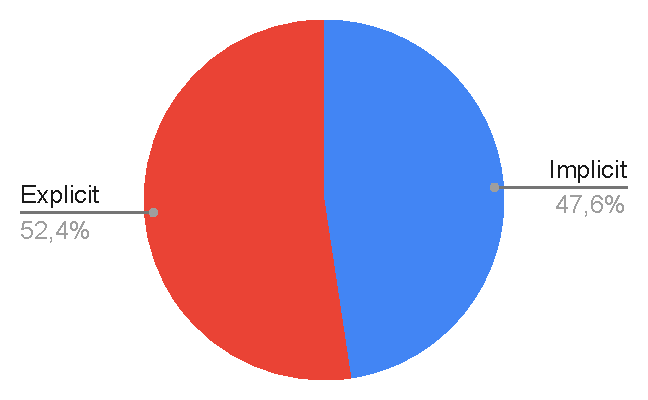
\includegraphics[width=10cm]{definition-academic.pdf}
  \end{center}
\end{figure}

\begin{figure}[H]
  \caption{Implicit vs. explicit definition of Developer Experience in grey literature}
  \begin{center}
    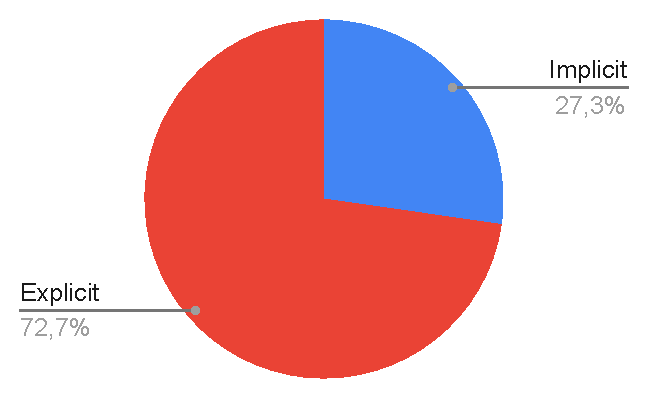
\includegraphics[width=10cm]{definition-grey.pdf}
  \end{center}
\end{figure}

\subsubsection{Context of DX}

From the analysis of the material, there is a clear indication that there are different viewpoints to Developer Experience.

Grey literature takes to a large degree a viewpoint where DX is a form of UX, where developers are users of products and services. In this viewpoint the DX consists of features that are also used when measuring the UX of a service. These include factors like functionality, usability, and reliability.

The grey literature is also heavily influenced by businesses marketing their services or products. To gain visibility and recognition, they are publishing articles and posts on their blogs to write and discuss a specific topic. These businesses are defining DX from their own point of view where they are providing products and services, that are directly used by developers.

Some articles (which?) mentioned that back in the days, it was executives that made the business and purchase decisions of tools, frameworks and other products and the developer's opinion were not considered. Developers were forced to use whatever they were offered.

Today, the purchase decision has more and more shifted to be a responsibility of the developer. Developers are the final users of the product and therefore businesses have probably realized that developers are the ones to make the decisions. All in all, it can be seen from the current grey literature that developers are being considered more and more (Devs are people too), and that this movement has created the concept of DX.

DX allows developers to reason about things that before has been difficult. Making statements that are in the favour of developers might have been difficult as there hasn't been any term to coin the feelings, emotions, needs,

Businesses have taken notice on this movement, and are now utilizing it to create products and services.

DX can be seen that there is always a developer that is a user. The role of the user is the variable, and can vary from being a user of a product where the DX is seen in the product, or then the user can be a user of a developer workflow in a software project.

In many of the grey literature articles the authors have their own view and definition of what DX is. Only in few articles there is actual questioning of the definition of DX.

The formal research on DX has taken a step further and is also considering the social aspects of software development.

A research group in Brazil has to a large extent researched the DX in the context of Mobile Software Ecosystems (MSECO). To these ecosystems belong mobile application development platforms as Android and iOS. Their approach to DX can however be seen as something applicable to all kinds of products and services that aim to create a better DX and improve on it.

Another group of researchers in Finland have studied the mood of developers and its effects at varying levels of software development.

Overall the amount of formal research on DX is lacking. The lack of definitions and the amount of search results in the search speaks for this.


Many articles use the keyword developer experience but only mention DX briefly in their material. This forces the readers to

\begin{table}[H]
  \begin{center}
    \begin{tabular}{l r}
      Definition                        & 5  \\
      Development Environment           & 11 \\
      API                               & 10 \\
      Product or service                & 9  \\
      User Experience                   & 14 \\
      Team, Collaboration, \& Community & 16 \\
      Mood \& Feelings                  & 8  \\
    \end{tabular}
    \caption{Academic and grey literature}
  \end{center}
\end{table}

\begin{table}[H]
  \begin{center}
    \begin{tabular}{l r}
      Definition                        & 4  \\
      Development Environment           & 9  \\
      API                               & 4  \\
      Product or service                & 2  \\
      User Experience                   & 7  \\
      Team, Collaboration, \& Community & 11 \\
      Mood \& Feelings                  & 7  \\
    \end{tabular}
    \caption{Academic literature}
  \end{center}
\end{table}

\begin{table}[H]
  \begin{center}
    \begin{tabular}{l r}
      Definition                        & 1  \\
      Development Environment           & 2  \\
      API                               & 6  \\
      Product or service                & 7  \\
      User Experience                   & 7  \\
      Team, Collaboration, \& Community & 5  \\
      Mood \& Feelings                  & 1  \\
    \end{tabular}
    \caption{Grey literature}
  \end{center}
\end{table}

\begin{figure}[H]
  \caption{Combined}
  \begin{center}
    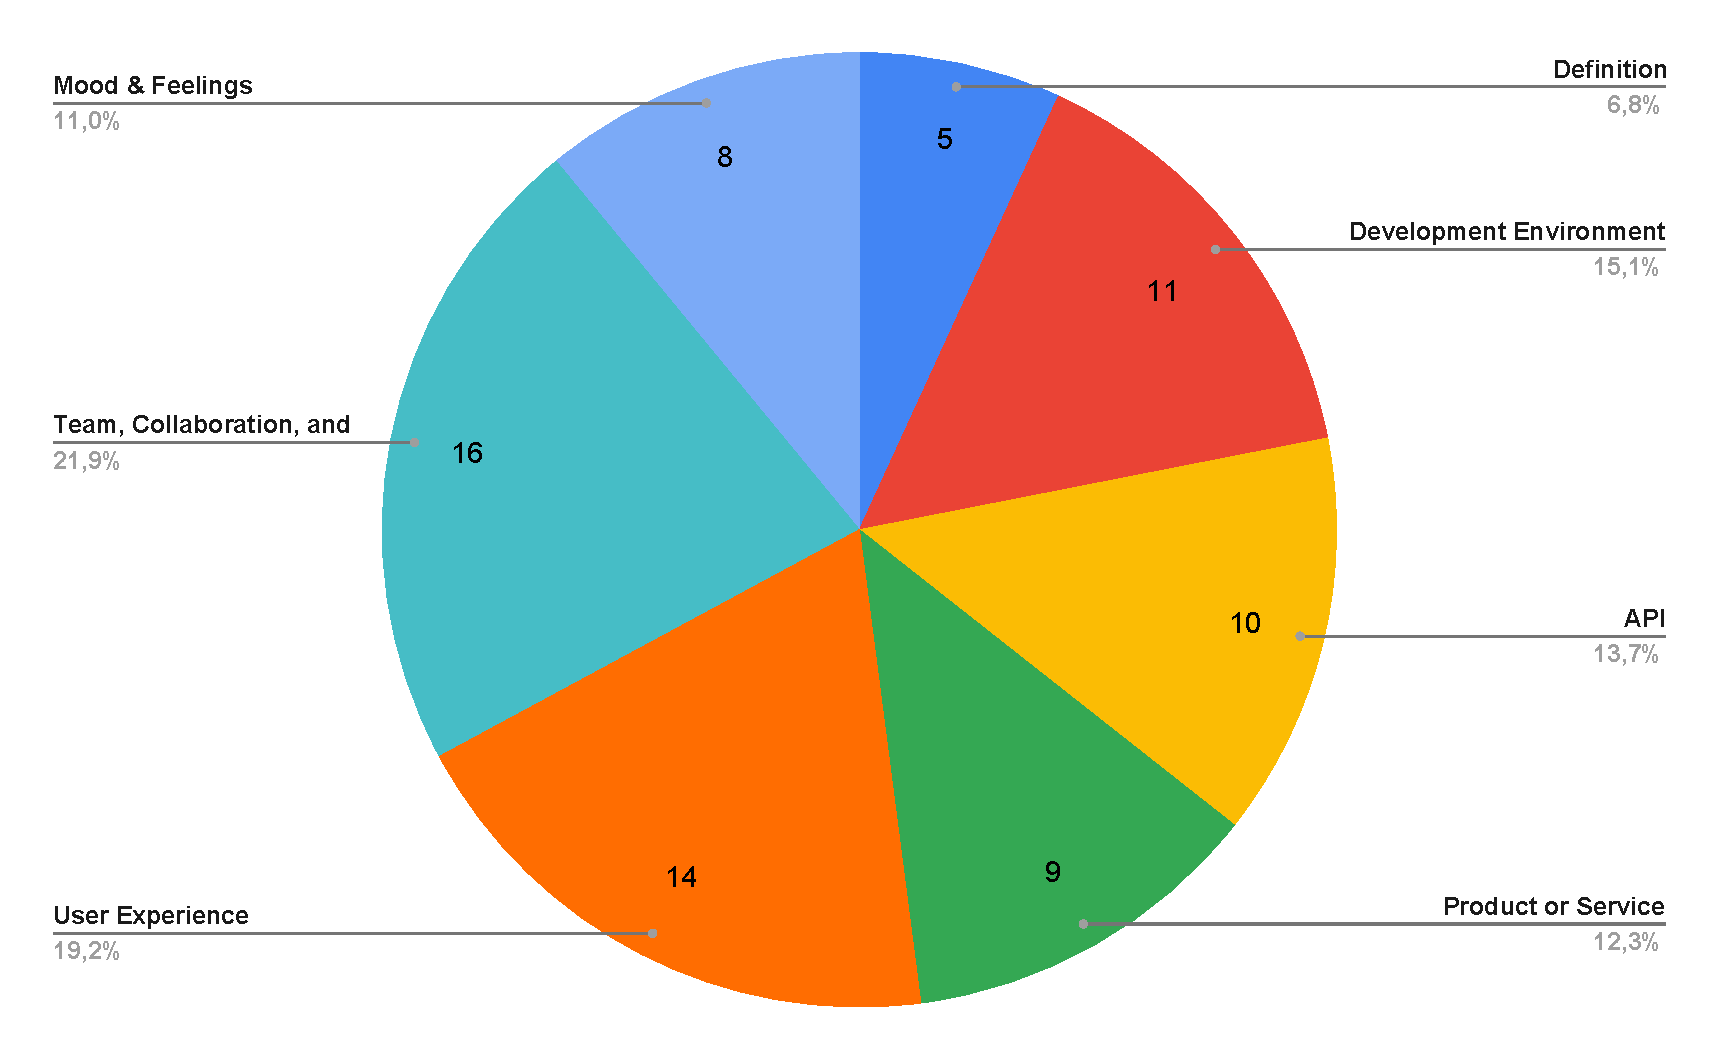
\includegraphics[width=\textwidth]{context-combined.pdf}
  \end{center}
\end{figure}

\begin{figure}[H]
  \caption{Academic}
  \begin{center}
    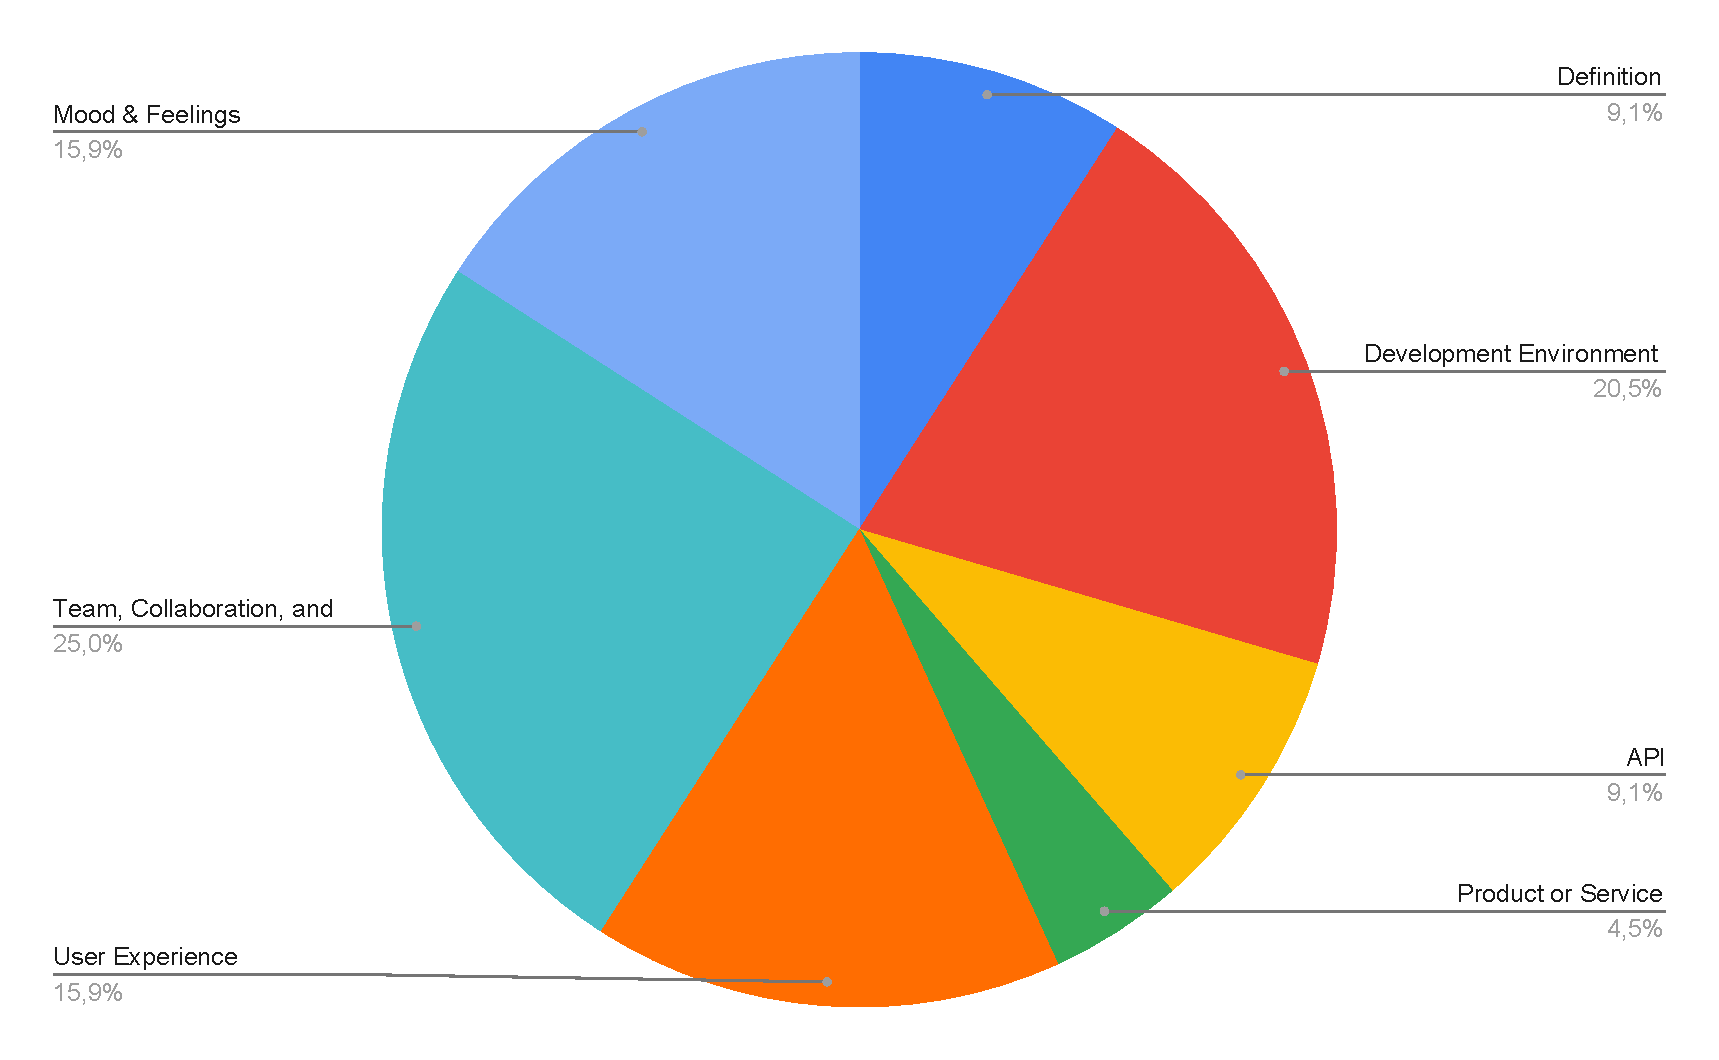
\includegraphics[width=\textwidth]{context-academic.pdf}
  \end{center}
\end{figure}

\begin{figure}[H]
  \caption{Grey}
  \begin{center}
    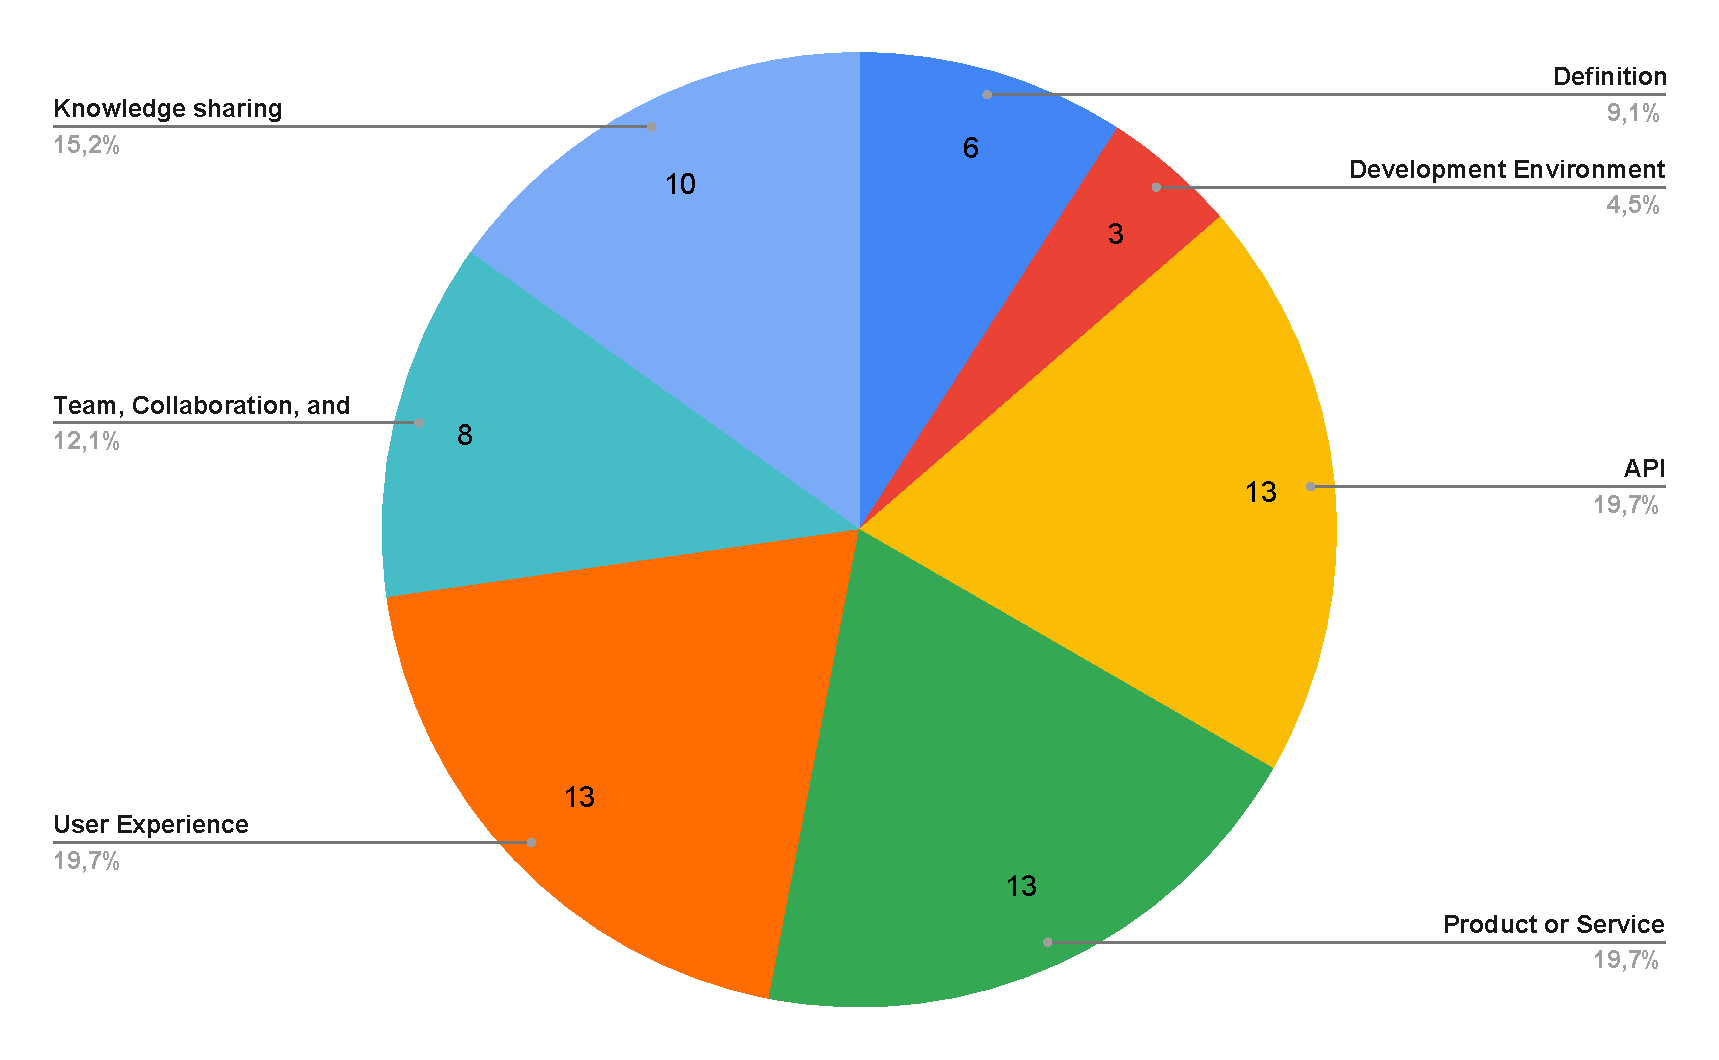
\includegraphics[width=\textwidth]{context-grey.pdf}
  \end{center}
\end{figure}

\subsection{Validity of search results}

The search engine Google is known to provide results based on many different variables on the user e.g. previous searchers, internet profile etc. Therefore the search results from Google might not present results that are applicable for anyone. To mitigate this, private sessions were used when performing the searches.

\clearpage
\section{Interviews and case studies}

Define what kind of practical approach to the study subject is going to be taken

\textbf{\\ Possible approaches for the practical part of the study:}

\newcommand{\uxdesigndx}{https://uxdesign.cc/contributing-great-developer-experience-designer-e1f497b0fb4}

\begin{itemize}
  \item [--] Based on the \href{\uxdesigndx}{this article}, create a set of guidelines and good practices of DX, and interview and/or measure how well established the application of the practices are
  \item [--] An interview studying the development environments of different projects. \href{\uxdesigndx}{\textit{"When starting a new project, be upfront that you want to tailor your tools and methods for collaboration"}}
  \item [--]
\end{itemize}

\clearpage
\section{Results}

Answer the research questions and problem.

\subsection{Validity of results}

T\"ass\"a osassa on syyt\"a my\"os arvioida tutkimustulosten luotettavuutta.
Jos tutkimustulosten merkityst\"a arvioidaan >>Tarkastelu>>-osassa,
voi luotettavuuden arviointi olla my\"os siell\"a.

\clearpage
\section{Summary}

\clearpage
\section{Conclusions}

\clearpage
\section{Possible references}

\textbf{SLR and MLR}
\begin{enumerate}
  \item K. M. Benzies, S. Premji, K. A. Hayden, and K. Serrett, "State-of-the-Evidence Reviews: Advantages and Challenges of Including Grey Literature,"Worldviews on Evidence-Based Nursing, vol. 3, pp. 55-61, 2006.
  \item Rucinski, Taryn. (2015). The Elephant in the Room: Toward a Definition of Grey Legal Literature. Law library journal. 107. 543.
  \item Joachim Schöpfel. Towards a Prague Definition of Grey Literature. Twelfth International Conference on Grey Literature: Transparency in Grey Literature. Grey Tech Approaches to High Tech Issues. Prague, 6-7 December 2010, Dec 2010, Czech Republic. pp.11-26.
  \item B. Kitchenham and S. Charters, "Guidelines for Performing Systematic Literature Reviews in Software engineering," in "EBSE Technical Report," 2007, vol. EBSE- 2007-01.
  \item V. Garousi, M. Felderer, Experience-based guidelines for effective and efficient data extraction in systematic reviews in software engineering, in: International Conference on Evaluation and Assessment in Software Engineering, Karlskrona, Sweden, 2017, pp. 170–179.
  \item Lotto, L. S. (1986). Qualitative Data Analysis: A Sourcebook of New Methods: Matthew B. Miles and A. Michael Huberman. Educational Evaluation and Policy Analysis, 8(3), 329–331. https://doi.org/10.3102/01623737008003329
  \item Using argumentation theory to analyse software practitioners’ defeasible evidence, inference and belief
        Author links open overlay panel. Austen Rainer
\end{enumerate}

\textbf{Development tools}
\begin{enumerate}
  \item Murphy,G.C.,Kersten,M.,Findlater,L.:HowareJavasoftwaredevelopersusingtheElipseIDE? Softw. IEEE 23(4), 76–83 (2006)
  \item 17. Muslu,K.,Brun,Y.,Holmes,R.,Ernst,M.D.,Notkin,D.:Speculative analysis of integrated development environment recommendations. ACM SIGPLAN Not. 47(10), 669–682 (2012)
  \item Kersten, M., Murphy, G.C.: Using task context to improve programmer productivity. In: Proceedings of the 14th ACM SIGSOFT International Symposium on Foundations of Software Engineering (SIGSOFT 2006/FSE-14), pp. 1–11. ACM, New York, NY, USA (2006)
  \item The Impact of "Cosmetic" Changes on the Usability of Error Messages Tao Dong, Kandarp Khandwala May 2019 CHI EA '19: Extended Abstracts of the 2019 CHI Conference on Human Factors in Computing Systems
  \item Designing a live development experience for web-components Jens Lincke, Patrick Rein, Stefan Ramson, Robert Hirschfeld, Marcel Taeumel, Tim Felgentreff October 2017 PX/17.2: Proceedings of the 3rd ACM SIGPLAN International Workshop on Programming Experience
  \item Are Software Developers Just Users of Development Tools? Assessing Developer Experience of a Graphical User Interface Designer. Kati Kuusinen Conference paper First Online: 23 August 2016
\end{enumerate}

\textbf{Software Development}
\begin{enumerate}
  \item Capretz, L.F., Ahmed, F.: Making sense of software development and personality types. IT Prof. 12(1), 6–13 (2010)
  \item An exploratory study on the influence of developers in technical debt Reem Alfayez, Pooyan Behnamghader, Kamonphop Srisopha, Barry Boehm May 2018 TechDebt '18: Proceedings of the 2018 International Conference on Technical Debt
\end{enumerate}

\textbf{Soft skills}
\begin{enumerate}
  \item empty
\end{enumerate}

\textbf{Developer mood}
\begin{enumerate}
  \item Graziotin, D., Wang, X., Abrahamsson, P.: Happy software developers solve problemsbetter: psychological measurements in empirical software engineering. PeerJ2(1), e289(2014)
  \item Beecham, S., Baddoo, N., Hall, T., Robinson, H., Sharp, H.: Motivation in software engineering: A systematic literature review. IST 50, 860–878 (2008)
  \item D. Graziotin, Consequences of unhappiness while developing software, in Proc. 2nd Int. Workshop Emotion Awareness Softw. Eng., May 2017, pp. 42–47.
  \item On the Unhappiness of Software Developers Daniel Graziotin, Fabian Fagerholm, Xiaofeng Wang, Pekka Abrahamsson June 2017 EASE'17: Proceedings of the 21st International Conference on Evaluation and Assessment in Software Engineering
\end{enumerate}

\textbf{Flow state and distractions. Sociability and Social Support}
\begin{enumerate}
  \item Ryan, R.M., Mims, V., Koestner, R.: Relation of reward contingency and interpersonal context to intrinsic motivation: a review and test using cognitive evaluation theory. J. Pers. Soc. Psychol. 45, 736–750 (1983)
  \item 27.Oehlberg,  L.,  Ducheneaut,  N.,  Thorton,  J.D.,  Moore,  R.J.,Nickell,  E.  2006.  Social  TV:  Designing  for  D istributed,  SocialTelevision Viewing. In Proc. Euro iTV’06. (2006), 251-259
  \item Leont’ev,  A.  N.  Activity,  consciousness,  and  personality.  Prentice-Hall Press, (1978)
  \item Perlow, L.A., The time famine: Toward a sociology of work time. Admin. Science Quarterly, 44, (1999), 57-81
\end{enumerate}

\textbf{User Experience}
\begin{enumerate}
  \item Hassenzahl, M., Tractinsky, N.: User experience - a research agenda. Behav. Inf. Technol. 25(2), 91–97 (2006)
  \item Henrique Henriques, Hugo Lourenço, Vasco Amaral, and Miguel Goulão. 2018. Improving the Developer Experience with a Low-Code Process Modelling Language. In Proceedings of the 21th ACM/IEEE International Conference on Model Driven Engineering Languages and Systems (MODELS '18). ACM, New York, NY, USA, 200-210. DOI: https://doi.org/10.1145/3239372.3239387
  \item Ferreira, J. , Sharp, H. and Robinson, H. (2011), User experience design and agile development: managing cooperation through articulation work. Softw: Pract. Exper., 41: 963-974. doi:10.1002/spe.1012
\end{enumerate}

\textbf{Other}
\begin{enumerate}
  \item Kansala, M. and Tuomivaara, S. (2013). Do Agile Principles and Practices Support the Well-being at Work of Agile Team Members? In Proceedings of the 8th International Conference on Software Engineering Advances (ICSEA 2013), pages 364–367.
  \item Dingsøyr, T., Nerur, S., Balijepally, V., and Moe, N. B. (2012). A decade of agile methodologies: Towards explaining agile software development. Journal of Systems and Software, 85(6):1213–1221.
  \item Journal of Systems and Software Volume 140, June 2018, Pages 32-47 Journal of Systems and Software What happens when software developers are (un)happy Author links open overlay panel Daniel Graziotina Fabian Fagerholm bcXiaofengWangd PekkaAbrahamssone Show more https://doi.org/10.1016/j.jss.2018.02.041
  \item Teamwork quality and project success in software development: A survey of agile development teams Author links open overlay panelYngveLindsjørnaDag I.K.Sjøbergab TorgeirDingsøyrbc Gunnar R.Bergersen Tore Dybåa
  \item Gass, O., Meth, H., Maedche, A.: PaaS characteristics for productive software development: an evaluation framework. Internet Comput. IEEE 18(1), 56–64 (2014)
  \item Deci, E., Ryan, R.M.: Self-determination theory. Handbook of theories of social psychology. SAGE, Los Angeles (2012). ISBN 9780857029607
\end{enumerate}

\clearpage
\thesisbibliography
\bibliography{thesis}
% Different bibliography styles can be found from https://www.overleaf.com/learn/latex/Bibtex_bibliography_styles
\bibliographystyle{abbrv}

\end{document}
